
\chapter{Application Description}

In this chapter present the application using code snippets, diagrams.

\section{Architecture}

The application uses a combination of Event Driven architecture and Request-Response architecture, making as much use as possible of Node JS's built in capabilities for handling multiple operations on a single thread using concurrency and asynchronous programming.

The application consists of multiple microservices. These microservices implement communication patterns like \textit{Request-Response} and \textit{Publish/Subscribe}. All microservice communication is done using message queues like RabbitMQ and BullMQ. While RabbitMQ offers great support for both Request-Response communication and Publish/Subscribe communication, I chose to use BullMQ for Publish/Subscribe. BullMQ uses Redis to queue messages and process them. By using Redis, BullMQ offers an easy way to schedule the times when a message is executed and implement retry policies. On the other hand, RabbitMQ is built upon AMQP (Advanced Message Queuing Protocol). This makes it possbile to pass messsages across an internal network and register handlers for these messages. 

Since this application is heavily focused on microservices, here is a short description for each one of them:
\begin{itemize}
    % \item Client - User interface, hosted on a server of its own.
    \item \textbf{Webserver Service} - Single HTTP server, tasked with serving the client application and providing HTTP routes for fetching data.
    \item \textbf{Authentication Service} - Service handling all authentication logic. This server is only accessible via RabbitMQ queues.
    \item \textbf{Core Service} - Service handling all reads and writes to the database. This server is accessbile via RabbitMQ queues.
    \item \textbf{Authorization Service} - Service handling authorization across the whole application. The application implements a RBAC (Role Based Access Control). Each request goes through this service before reaching the Core service. Only accessbile via RabbitMQ.
    \item \textbf{Uploader Service} - Service handling all file uploads. Since uploads are usually resource intensive tasks and can fail due to numerous reasons, this is a processor service using BullMQ.
    \item \textbf{Mail Service} - Service handling all emails sent. Sending emails is also a resource intensive task especially if sending to multiple users at the same tim. This is a processor service using BullMQ.
    \item \textbf{Websocket Server} - Server exposing only a websocket connection. This server is handling all of the chat features inside of the application, listening for notifications sent by clients, invoking the Core service for different writes (saves, updates) to the database, and dispatching a notification to the intended client.
    \item \textbf{Notification Server} - Server exposing a route for handling SSE (Server Sent Events). This server is the one handling in-app notifications. 
\end{itemize}

Authentication Logic (e.g. Figure \ref{fig:authLogic}).

File upload Logic (e.g Figure \ref{fig:uploaderLogic}).

Use Case Diagram (e.g Figure \ref{fig:useCase}).
\begin{figure}[!ht]
    \centering
    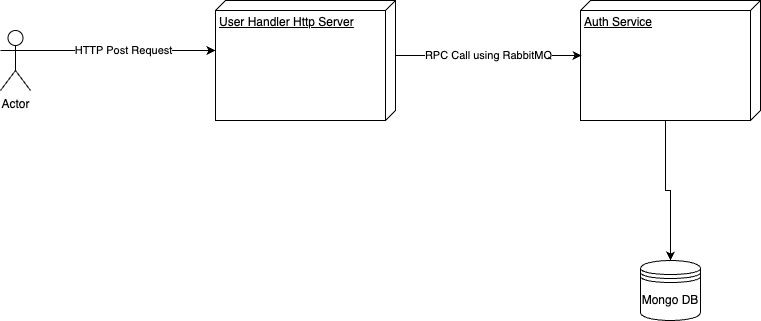
\includegraphics[width=1\linewidth]{login.drawio.png}
    \caption{Authentication Logic Diagram}
    \label{fig:authLogic}
\end{figure}

\begin{figure}[!ht]
    \centering
    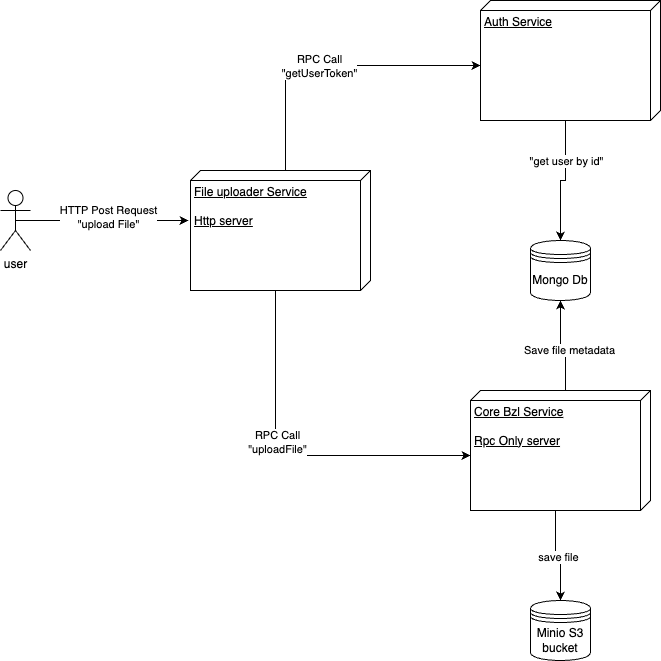
\includegraphics[width=1\linewidth]{file uplaod.drawio.png}
    \caption{File Uploader Logic Diagram}
    \label{fig:uploaderLogic}
\end{figure}

\begin{figure}[!ht]
    \centering
    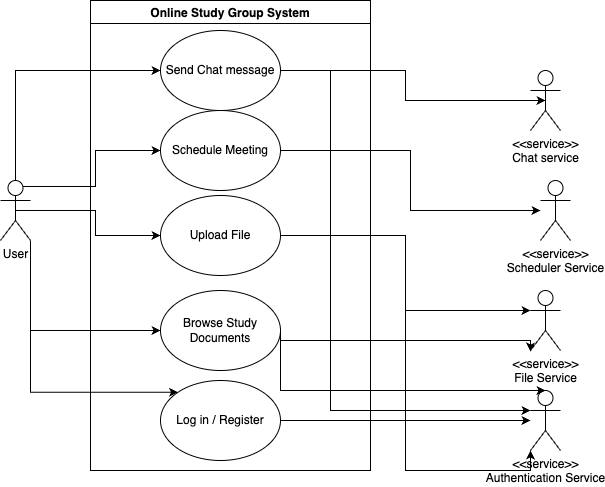
\includegraphics[width=1\linewidth]{Use Case Licenta.drawio.png}
    \caption{Use Case Diagram}
    \label{fig:useCase}
\end{figure}

\newpage
\section{Features}
The main features of the application are: a steady authentication, a live-chat for allowing students to study in groups and a file-sharing system for easily sharing study notes.

\subsection{Authentication}
The most important part of any web based application is the authentication. While developing the authentication system for my application, I followed OAuth2 standards. 

\textbf{Registration}: During registration, users submit their full name, email, password and a confirmation password. The system hashes the password with a strong algorithm (implemented using bcryptjs), creates a new user record marked as unverified, and generates a time-limited email verification token. The token is stored in the database and emailed, prompting users to confirm their address.

Endpoint: /auth/register

Method: POST

Request Body: JSON Object containing fullname, email, password and confirmation password.

Response: JSON Object containing a success message if the request was successful

\textbf{Verify Account}: When users click the verification link, the system extracts the token and searches the database for a matching, unexpired record. If valid, it marks the user’s account as verified, removes the token to prevent reuse, and returns a success response, enabling full access to login and other protected features.

Endpoint: /auth/verifyaccount

Method: GET

Query Parameters: verificationToken (string) -> verification token for certain account, recieved via email.

Response: JSON Object containing a success message if the request was successful


\textbf{Login}: On login, users submit credentials, which the system verifies against stored hashes. After confirming the account is verified, it generates a cryptographically secure session code, encrypts it, and stores it in the database under the user profile. The code is set in an HttpOnly, Secure cookie, establishing the authenticated session.

Endpoint: /auth/login

Method: POST

Request Body: JSON Object containing email, and password.

Response: JSON Object containing a success message if the request was successful.

\textbf{Reset Password}: When a password reset is requested, users provide their email address. The system generates a short-lived, cryptographically random reset token, stores it, and emails a reset link. Upon visiting the link and submitting a new password, the system validates the token, updates the password hash and deletes the token.

Endpoint: /auth/reset-password

Method: POST

Request Body: JSON Object containing reset token, password and confirmation password.

Response: JSON Object containing a success message if the request was successful


\textbf{Logout}: For logout, the client sends a request to invalidate the session. The server locates the encrypted session code in the database, removes it, and instructs the browser to clear the authentication cookie by setting it with a past expiration. The user is then unauthenticated for any subsequent requests.

Endpoint: /auth/logout

Method: POST

Response: JSON Object containing a success message if the request was successful.

\textbf{Whoami}: For Whoami, the client sends a request to get the user holding the current session. The server locates the encrypted session code in the database, and returns the user data.

Endpoint: /auth/whoami

Method: Get

Response: JSON Object containing userId, role and email of the logged in user if the request was successful.

\subsection{Live-chat}

\section{Technology Stack}
Since this is a web browser based application,it mainly consists of JavaScript/TypeScript code on the client side. However, due to JavaScript`s asynchronous nature, and the different microservices that must handle asynchronous operations, the server side code is also implemented in JavaScript/TypeScript.
\subsection{Server Implementation}
The server for 'Cloud Class' contains all of the logic at the backbone of the application, offering a solid foundation for the client`s app functionalities.

\begin{itemize}
    \item \textbf{Programming Language:} \textit{TypeScript} - TypeScript is a statically typed superset of JavaScript that compiles down to plain JavaScript. It introduces optional type annotations, interfaces, and advanced tooling for improved code quality, maintainability, and developer productivity, enabling safer large-scale application development.
    \item \textbf{Runtime Environment:} \textit{Node.js} - Node.js is a cross-platform, event-driven JavaScript runtime built on Chrome’s V8 engine. It uses non-blocking I/O and an event loop to efficiently handle concurrent connections, making it ideal for scalable network applications, microservices, and real-time servers.
    \item \textbf{Framework:} \textit{Nest.js} - NestJS is a progressive Node.js framework built with TypeScript, leveraging decorators and dependency injection to structure applications into modular, testable components. It abstracts common server-side patterns, integrates seamlessly with Express or Fastify, and supports GraphQL, WebSockets, and microservices out of the box.
    \item \textbf{Database:} \textit{MongoDB} - MongoDB is a document-oriented NoSQL database that stores data in flexible, JSON-like BSON documents. It offers horizontal scalability through sharding, built-in replication for high availability, and a powerful query language. MongoDB suits dynamic schemas, real-time analytics, and modern web or mobile applications.
    \item \textbf{Storage:} \textit{MinIO S3} -MinIO is a high-performance, Kubernetes-native object storage server compatible with the Amazon S3 API. It provides erasure coding, bitrot protection, and encryption for secure, scalable storage. MinIO excels in private cloud or edge deployments, supporting multi-tenancy and lightweight resource footprints.
    \item \textbf{Real Time Communication:} \textit{Socket.IO and Server Sent Events (SSE)} - Socket.IO enables real-time, bidirectional communication between clients and servers over WebSockets and fallback transports, ideal for chat, gaming, or live updates. Server-Sent Events (SSE) provide unidirectional, low-overhead streams from server to browser. Both facilitate reactive interfaces and event-driven architectures.
    \item \textbf{Logging:} \textit{Elastic Search} - Elasticsearch is a distributed, RESTful search and analytics engine built on Apache Lucene. It indexes documents for lightning-fast full-text, structured, and geo-queries. Elasticsearch scales horizontally, supports real-time data ingestion, and powers features like autocomplete, logging pipelines, and business intelligence dashboards.
    \item \textbf{Testing:} \textit{Jest} - Jest is a delightful JavaScript testing framework maintained by Facebook. It offers zero-configuration setup, snapshot testing, and built-in mocking utilities. Jest runs tests in parallel for speed and provides rich watch-mode feedback, making test-driven development smooth for React, Node.js, and beyond.
    \item \textbf{Message Queues:} \textit{RabbitMQ and BullMQ} - RabbitMQ is an open-source message broker implementing AMQP. It offers flexible routing, message acknowledgments, clustering, and high availability. Through plugins and management UI, you can monitor queues and extend functionality. RabbitMQ enables reliable, asynchronous communication between distributed applications and microservices. BullMQ is a Node.js library for robust background job processing using Redis. With a TypeScript-first API, it supports job queues, workers, rate limiting, repeatable jobs, and atomic operations. BullMQ ensures reliable task scheduling for use cases like email delivery, data pipelines, and notification dispatch.
\end{itemize}

\subsection{Client Implementation}
The client application for 'Cloud Class' offers a easy-to-use interface, allowing users to collaborate easily with each other. 


\begin{itemize}
    \item \textbf{HTML:} - HTML (Hyper Text Markup Language) is the standard markup language for creating web pages. It structures content using elements like headings, paragraphs, links, and media embeds. Semantic tags improve accessibility and SEO, while forms and tables enable user input and data presentation, forming the backbone of every website.
    \item \textbf{CSS:} - CSS (Cascading Style Sheets) styles and layouts HTML content, controlling colors, typography, spacing, and responsive behavior. With selectors, properties, and media queries, it allows designs to adapt across devices. Modern features like Flexbox, Grid, and custom properties enable complex, maintainable, and dynamic user interfaces with minimal code.
    \item \textbf{React:} - React is a JavaScript library for building component-based user interfaces. It uses a virtual DOM for efficient updates and a declarative syntax with JSX. React’s ecosystem includes hooks for state and side effects, and tools like React Router and Redux, making it ideal for complex, interactive web apps.
    \item \textbf{Socket.IO:} - React is a JavaScript library for building component-based user interfaces. It uses a virtual DOM for efficient updates and a declarative syntax with JSX. React’s ecosystem includes hooks for state and side effects, and tools like React Router and Redux, making it ideal for complex, interactive web apps.
\end{itemize}

% \begin{defn} Angular
% \end{defn}
% \begin{defn} Node JS
% \end{defn}
% \begin{defn} Minio S3
% \end{defn}
% \begin{defn} Mongo DB
% \end{defn}
% \begin{defn} Rabbit MQ
% \end{defn}

\section{References}
The bibliography has to be referenced in thesis content using cite (e.g. \cite{Bersani}).

\section{Interface}
Present App interface using Screenshots?

Each figure has to have a caption that is a suggestive description of what  the  picture represents (e.g. Figure \ref{fig:siglaUVT}).
\begin{figure}[!ht]
    \centering
    
\includegraphics[width=0.25\linewidth]{FMI-03.png}
    \caption{ FMI logo scaled at 25\% of text width}
    \label{fig:siglaUVT}
\end{figure}

\section{Algorithm pseudo-code}
Present pseudo-code and actual code for a feature.

Pseudo-code is a formal way to describe an algorithm, is more clear than a textual description ore code ( e.g. Algorithn \ref{alg:alg_ex}).

\begin{algorithm}[!ht]
\caption{An algorithm with caption}\label{alg:alg_ex}
\begin{algorithmic}[1]
\Require $n \geq 0$
\Ensure $y = x^n$
\State $y \gets 1$
\State $X \gets x$
\State $N \gets n$
\While{$N \neq 0$}
\If{$N$ is even}
    \State $X \gets X \times X$
    \State $N \gets \frac{N}{2}$  \Comment{This is a comment}
\ElsIf{$N$ is odd}
    \State $y \gets y \times X$
    \State $N \gets N - 1$
\EndIf
\EndWhile
\end{algorithmic}
\end{algorithm}

\section{Adding code}
If it necessary to add  some code from the application, do not use print-screens, use  listing  (e.g. listing \ref{lst:p1}).
\begin{lstlisting}[language=Python, numbers=left,
    stepnumber=1, caption=Un exemplu de cod python, label=lst:p1]
import numpy as np
    
def incmatrix(genl1,genl2):
    m = len(genl1)
    n = len(genl2)
    M = None #to become the incidence matrix
    VT = np.zeros((n*m,1), int)  #dummy variable
    
    #compute the bitwise xor matrix
    M1 = bitxormatrix(genl1)
    M2 = np.triu(bitxormatrix(genl2),1) 

    for i in range(m-1):
        for j in range(i+1, m):
            [r,c] = np.where(M2 == M1[i,j])
            for k in range(len(r)):
                VT[(i)*n + r[k]] = 1;
                VT[(i)*n + c[k]] = 1;
                VT[(j)*n + r[k]] = 1;
                VT[(j)*n + c[k]] = 1;
                
                if M is None:
                    M = np.copy(VT)
                else:
                    M = np.concatenate((M, VT), 1)
                
                VT = np.zeros((n*m,1), int)
    
    return M
\end{lstlisting}

\section{Database Structure}

Present Strucutres for all database documents used in the application, using code snippets, diagrams, photos